\chapter{Z Tanım Bölgesinde Durum Geri Besleme Kontrolörü}
Durum uzay modeli
\begin{equation}
    x(k)=A x(k-1)+Bu(k-1),\quad y(k-1)=C x(k-1)
\end{equation}
olmak üzere 
\begin{equation}
    u(k-1)=K x(k-1)
\end{equation}
kontrolörüne \textbf{Durum Geri Besleme} kontrolörü adı verilmektedir. Dikkat edilirse bu kontrol kuralı
\begin{equation}
\begin{split}
    u(k-1)&=K x(k-1)\\
    u(k-1)&=\begin{bmatrix}k_1& k_2& \cdots& k_n\end{bmatrix} \begin{bmatrix}x_1(k-1)\\x_2(k-1)\\\vdots\\x_n(k-1)\end{bmatrix}\\
    u(k-1)&=k_1x_1(k-1)+k_2x_2(k-1)+\cdots+k_nx_n(k-1)
\end{split}
\end{equation}
olarak yazılabilir. Bu kontrolör ile kapalı çevrim durum uzay modeli
\begin{equation}
    \begin{split}
        x(k)&=A x(k-1)+Bu(k-1),\quad y(k-1)=C x(k-1)\\
        x(k)&=A x(k-1)+BKx(k-1),\quad y(k-1)=C x(k-1)\\
        x(k)&=(A+BK) x(k-1),\quad y(k-1)=C x(k-1)
    \end{split}
\end{equation}
olarak elde edilir. Kapalı çevrim modelin z tanım bölgesi ifadesi
\begin{equation}
    \begin{split}
        x(k)&=(A+BK) x(k-1)+B r(k-1),\quad y(k-1)=C x(k-1)\\
        z^1 x(k-1)&=(A+BK) x(k-1)+B r(k-1),\quad y(k-1)=C x(k-1)\\
        (zI-(A+BK)) x(k-1)&=B r(k-1),\quad y(k-1)=C x(k-1)\\
        x(k-1)&=(zI-(A+BK))^{-1} B r(k-1),\quad y(k-1)=C x(k-1)\\
        y(k-1)&=C(zI-(A+BK))^{-1}B r(k-1)\\
        \frac{y(k-1)}{r(k-1)}&=C(zI-(A+BK))^{-1}B
    \end{split}
\end{equation}
şeklindedir ve karakteristik polinom
\begin{equation}
    \begin{split}
        p_c(z)=det(zI-(A+BK))
    \end{split}
\end{equation}
ile hesaplanır. Bu polinom için kutuplar seçilirken $K$ kontrolör matrisi hesaplanır. Bu işlem için
\begin{equation}
    K=-\begin{bmatrix}0& 0& \cdots& 0& 1\end{bmatrix}\begin{bmatrix}B& AB& \cdots& A^{n-1}B\end{bmatrix}^{-1}p_d(A)
\end{equation}
burada $p_d(z)$ atanmak istenen polinom olmak üzere formülü kullanılabilir. 
\begin{equation}
    \begin{split}
\begin{bmatrix}
    x_1[k]\\
    x_2[k]
\end{bmatrix}&=
\begin{bmatrix}
    1& 0.1\\
    -0.1& 0.95
\end{bmatrix}\begin{bmatrix}
    x_1[k-1]\\
    x_2[k-1]
\end{bmatrix}+\begin{bmatrix}
    0\\
    0.1
\end{bmatrix}u[k-1]\\
y[k-1]&=\begin{bmatrix}
    1&0 
\end{bmatrix}\begin{bmatrix}
    x_1[k-1]\\
    x_2[k-1]
\end{bmatrix}\\
\end{split}
\end{equation}
ile verilen sistem için yerleşme zamanı $t_s=1,\,s$ ve aşım $\%10$ olacak şekilde bir durum geri besleme kontrolörü tasarlansın. Aday karakteristik polinom 
\begin{equation}
\begin{split}
    p_d(s)&=s^2+8s+45.7844\\
    &=(s+4 + 5.4575i)(s+4 - 5.4575i)
\end{split}
\end{equation}
şeklindedir ve z tanım Bölgesinde
\begin{equation}
    \begin{split}
        p_d(z)&=(z-0.57295-0.34794i)(z-0.57295+0.34794i)\\
        &=z^2 - 1.146z + 0.4493
    \end{split}
\end{equation}
şeklindedir. $p_d(A)$ terimi
\begin{equation}
    \begin{split}
        p_d(A)&=z^2 - 1.146z + 0.4493\bigg{|}_{z=A}\\
        &=A\cdot A - 1.146A + 0.4493I\\
        &=\begin{bmatrix} 0.99&0.195\\-0.195& 0.8925\end{bmatrix}-
        \begin{bmatrix}1.146&0.1146\\-0.1146&1.0887\end{bmatrix}+
        \begin{bmatrix}0.4493&0\\0&0.4493\end{bmatrix}\\
        &=\begin{bmatrix}0.2934&0.0804\\-0.0804&0.2532\end{bmatrix} 
    \end{split}
\end{equation}
olarak hesaplanır ve geri besleme kontrolörü
\begin{equation}
    \begin{split}
        K&=-\begin{bmatrix}0&1\end{bmatrix}\begin{bmatrix}0& 0.0100\\0.1& 0.0950\end{bmatrix}^{-1} \begin{bmatrix}0.2934&0.0804\\-0.0804&0.2532\end{bmatrix} \\
        &=\begin{bmatrix}-29.3433& -8.04104\end{bmatrix} 
    \end{split}
\end{equation}
olarak elde edilir. Durum uzayı modeli ve geri besleme kontrolörü ile birlikte Şekil~\ref{fig:lec12_model1} ile gösterilmiştir. 

\begin{figure}[!htb]
    \centering
    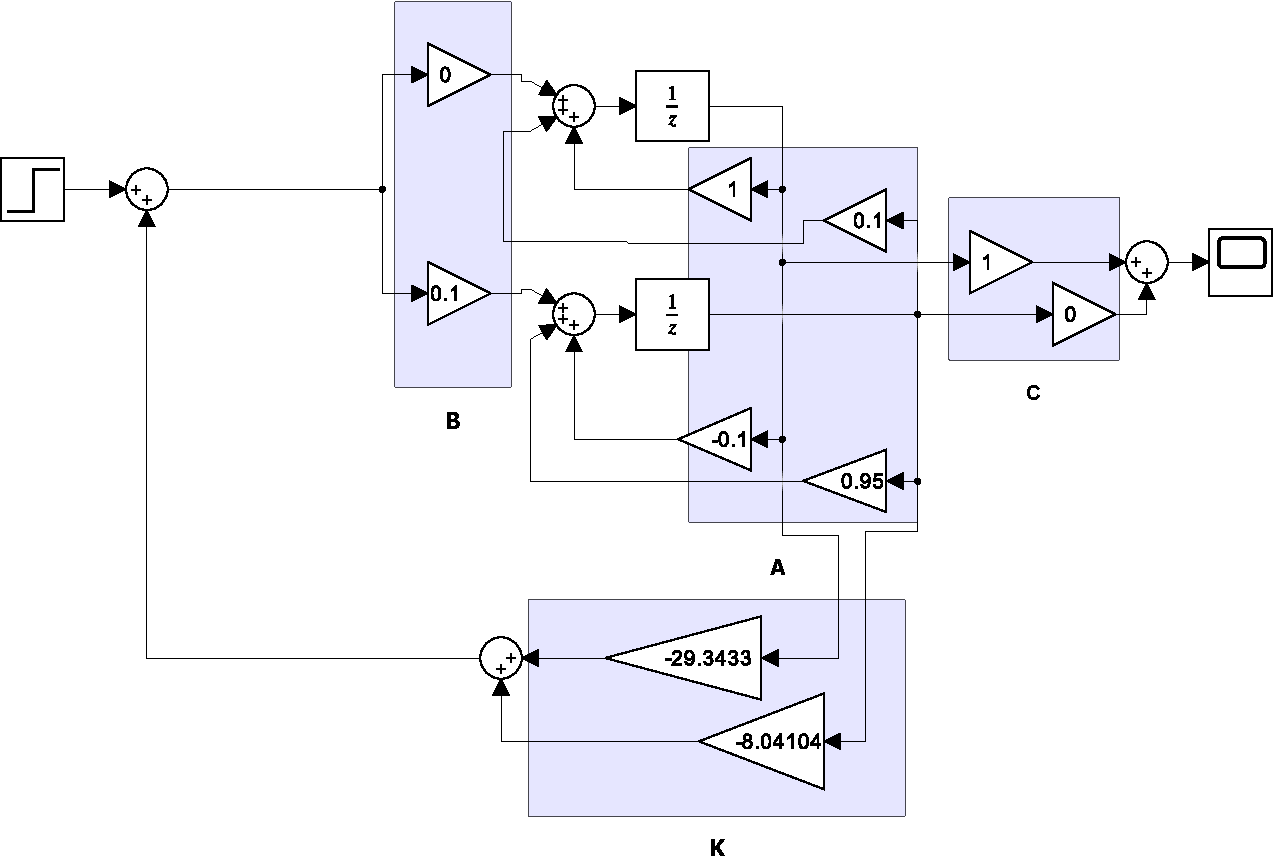
\includegraphics[width=\textwidth]{img/lec12_model1}
    \caption{Yay-kütle-damper sistemine ait ayrık durum uzay modeli ve geri besleme kontrolörü}
    \label{fig:lec12_model1}
\end{figure}


\begin{figure}[!htb]
    \centering
    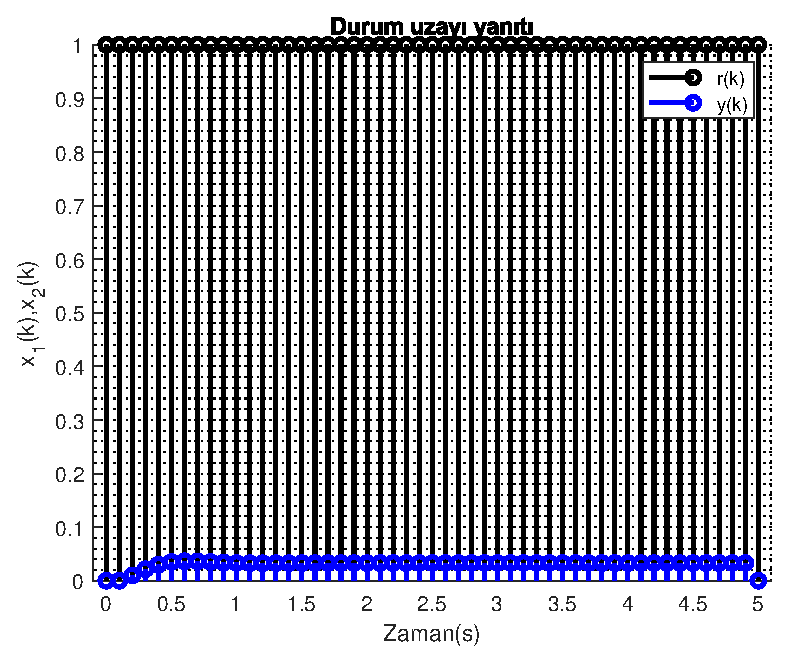
\includegraphics[width=0.75\textwidth]{img/lec12_plot1}
    \caption{Yay-kütle-damper sistemine ait ayrık durum uzay modeli ve geri besleme kontrolörü basamak yanıtı}
    \label{fig:lec12_plot1}
\end{figure}

\begin{figure}[!htb]
    \centering
    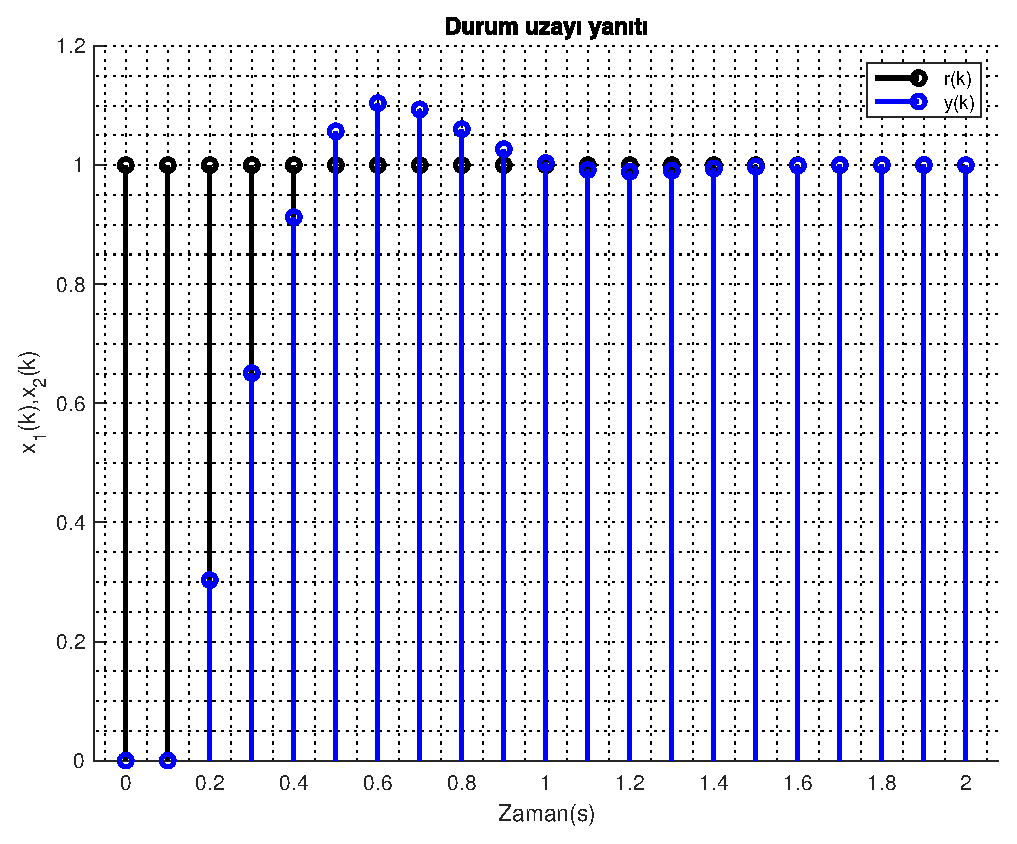
\includegraphics[width=0.75\textwidth]{img/lec12_plot2}
    \caption{Yay-kütle-damper sistemine ait ayrık durum uzay modeli ve geri besleme kontrolörü ön filtreli basamak yanıtı}
    \label{fig:lec12_plot2}
\end{figure}


